% Unidad 0. Herramientas matemáticas para Física y Química
%----------------------------------------------------------------------------------------
% A. Las destrezas científicas básicas
%   - Herramientas matemáticas básicas en diferentes escenarios científicos: potencias de 10
%     (significado, paso a decimal, multiplicación, división, cambio de lado de la raya de
%     fracción y potencia de una potencia), despeje de ecuaciones de primer grado (método de
%     operar en los dos miembros y método de "pasar" al otro lado, incógnita en el
%     denominador) y representación e interpretación de gráficas lineales (ejes con nombre de
%     magnitudes, "A vs B", pendiente y ordenada en el origen).
%
% Unidad de repaso: se trabaja como Unidad 0, antes de empezar las unidades de Química y Física.
%----------------------------------------------------------------------------------------

\spacing{1.3}
\raggedbottom % pages with large figures end where the text ends (no stretched gaps between boxes)

In physics and chemistry we use mathematics all the time: to write very big and very small numbers, to calculate a quantity from a formula, or to draw and read graphs. This unit is a \textbf{toolbox}: you can come back to it whenever you need to remember how something is done.

%----------------------------------------------------------------------------------------

\section{Powers of 10}

\subsection{What is a power of 10?}

\begin{definition}[Power of 10]
    A number of the form \(10^{n}\), where the \textbf{exponent} \(n\) is a whole number. It means that we multiply 10 by itself \(n\) times: \(10^{3} = 10 \cdot 10 \cdot 10 = 1000\).
\end{definition}

\begin{figure}[H]
    \centering
    % [FIGURA ORIGINAL] \includegraphics[width=\textwidth]{Unit_0/power10_line}
    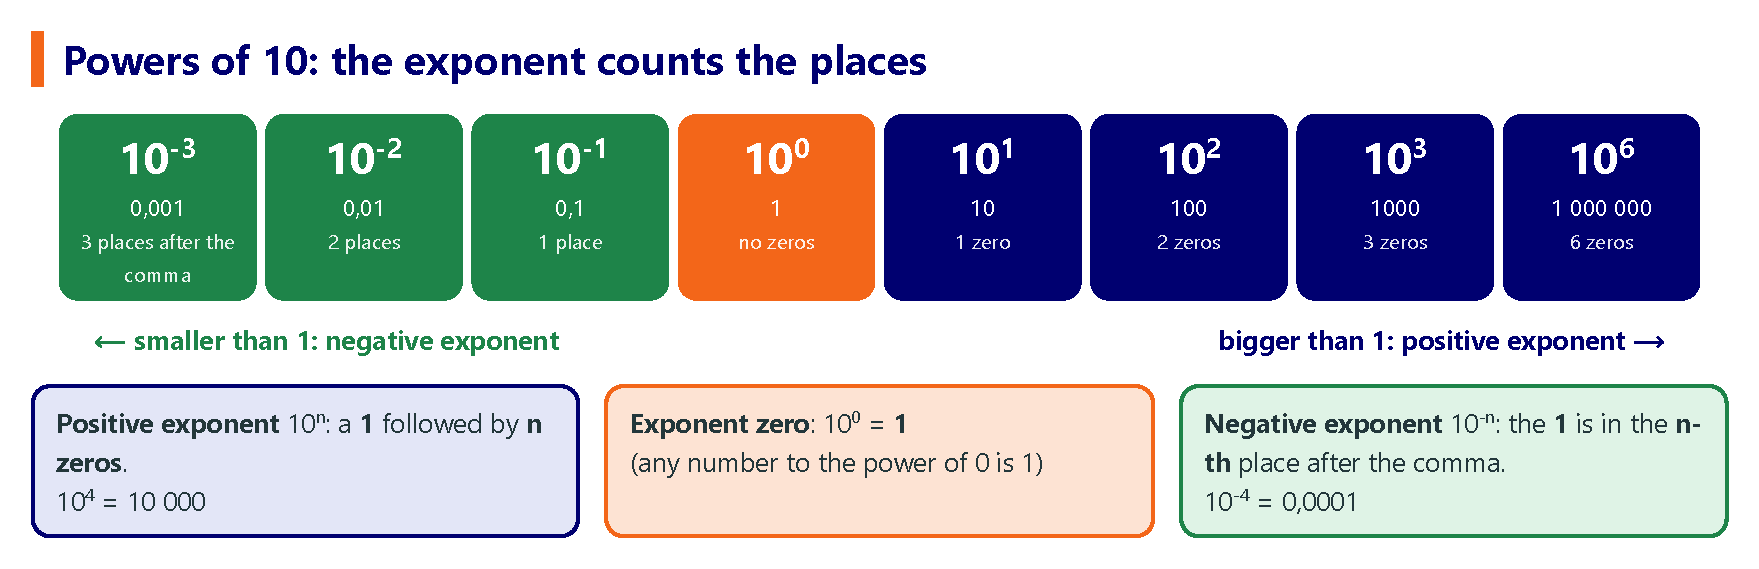
\includegraphics[width=\textwidth]{FigurasSVG/Unit_0_Math_Tools/pdf/power10_line.pdf}
    \caption{Positive exponents give numbers bigger than 1; negative exponents give numbers smaller than 1.}
    \label{fig:u0_power10_line}
\end{figure}

\begin{impt}
    \begin{itemize}
        \item \(10^{n}\) with \(n\) \textbf{positive}: a \textbf{1} followed by \textbf{\(n\) zeros}. \quad \(10^{5} = \num{100000}\).
        \item \(10^{0} = 1\).
        \item \(10^{-n}\) with \(n\) \textbf{positive}: a decimal number with the \textbf{1} in the \textbf{\(n\)-th place} after the comma. \quad \(10^{-5} = \num{0.00001}\).
    \end{itemize}
\end{impt}

\subsection{Writing numbers with powers of 10, and back to decimal}

Any number can be written as a number multiplied by a power of 10. It is still \textbf{the same number}, only written in a different way:
\begin{equation*}
    \num{5000} = 5 \cdot \num{1000} = 5 \cdot 10^{3}
    \qquad\qquad
    \num{0.007} = 7 \cdot \num{0.001} = 7 \cdot 10^{-3}
\end{equation*}

\negsubro{From a power of 10 to decimal}: the exponent tells us how many places the comma moves.
\begin{itemize}
    \item \textbf{Positive} exponent: the comma moves to the \textbf{right} (the number gets bigger). If there are no more digits, we add zeros: \(\num{3.2e4} = 3{,}2 \to 32\,000\).
    \item \textbf{Negative} exponent: the comma moves to the \textbf{left} (the number gets smaller). If there are no more digits, we add zeros and a 0 in front of the comma: \(\num{4.5e-3} = \num{0.0045}\).
\end{itemize}

\begin{example}
    \textbf{Write as a power of 10, and then go back to decimal.}
    \begin{itemize}
        \item \(\num{1000000} = 10^{6}\) (a 1 and six zeros). Back: \(10^{6}\) \(\to\) 1 followed by 6 zeros \(= \num{1000000}\).
        \item \(\num{0.01} = 10^{-2}\) (the 1 is in the 2nd place after the comma). Back: \(10^{-2} = \num{0.01}\).
        \item \(\num{80000} = 8 \cdot 10^{4}\). Back: \(8 \cdot 10^{4}\) \(\to\) the comma of 8 moves 4 places to the right: \(\num{80000}\).
        \item \(\num{0.0006} = 6 \cdot 10^{-4}\). Back: \(6 \cdot 10^{-4}\) \(\to\) the comma of 6 moves 4 places to the left: \(\num{0.0006}\).
    \end{itemize}
\end{example}

\begin{exercise}
    Write these numbers as a power of 10 (or as a number times a power of 10):
    \begin{enumerate}[label=\letraminuscula]
        \item \num{10000}
        \item \num{0.001}
        \item \num{100000000}
        \item \num{0.000001}
        \item \num{3000}
        \item \num{0.05}
        \item \num{7000000}
        \item \num{0.0009}
    \end{enumerate}
    \begin{solu}
        a) \(10^{4}\); b) \(10^{-3}\); c) \(10^{8}\); d) \(10^{-6}\); e) \(3 \cdot 10^{3}\); f) \(5 \cdot 10^{-2}\); g) \(7 \cdot 10^{6}\); h) \(9 \cdot 10^{-4}\).
    \end{solu}
\end{exercise}

\begin{exercise}
    Write these numbers as decimal numbers:
    \begin{enumerate}[label=\letraminuscula]
        \item \(10^{3}\)
        \item \(10^{-4}\)
        \item \(2 \cdot 10^{5}\)
        \item \(6{,}5 \cdot 10^{2}\)
        \item \(3 \cdot 10^{-2}\)
        \item \(1{,}2 \cdot 10^{-3}\)
    \end{enumerate}
    \begin{solu}
        a) \num{1000}; b) \num{0.0001}; c) \num{200000}; d) \num{650}; e) \num{0.03}; f) \num{0.0012}.
    \end{solu}
\end{exercise}

\subsection{The rules of powers of 10}

\begin{figure}[H]
    \centering
    % [FIGURA ORIGINAL] \includegraphics[width=\textwidth]{Unit_0/power10_rules}
    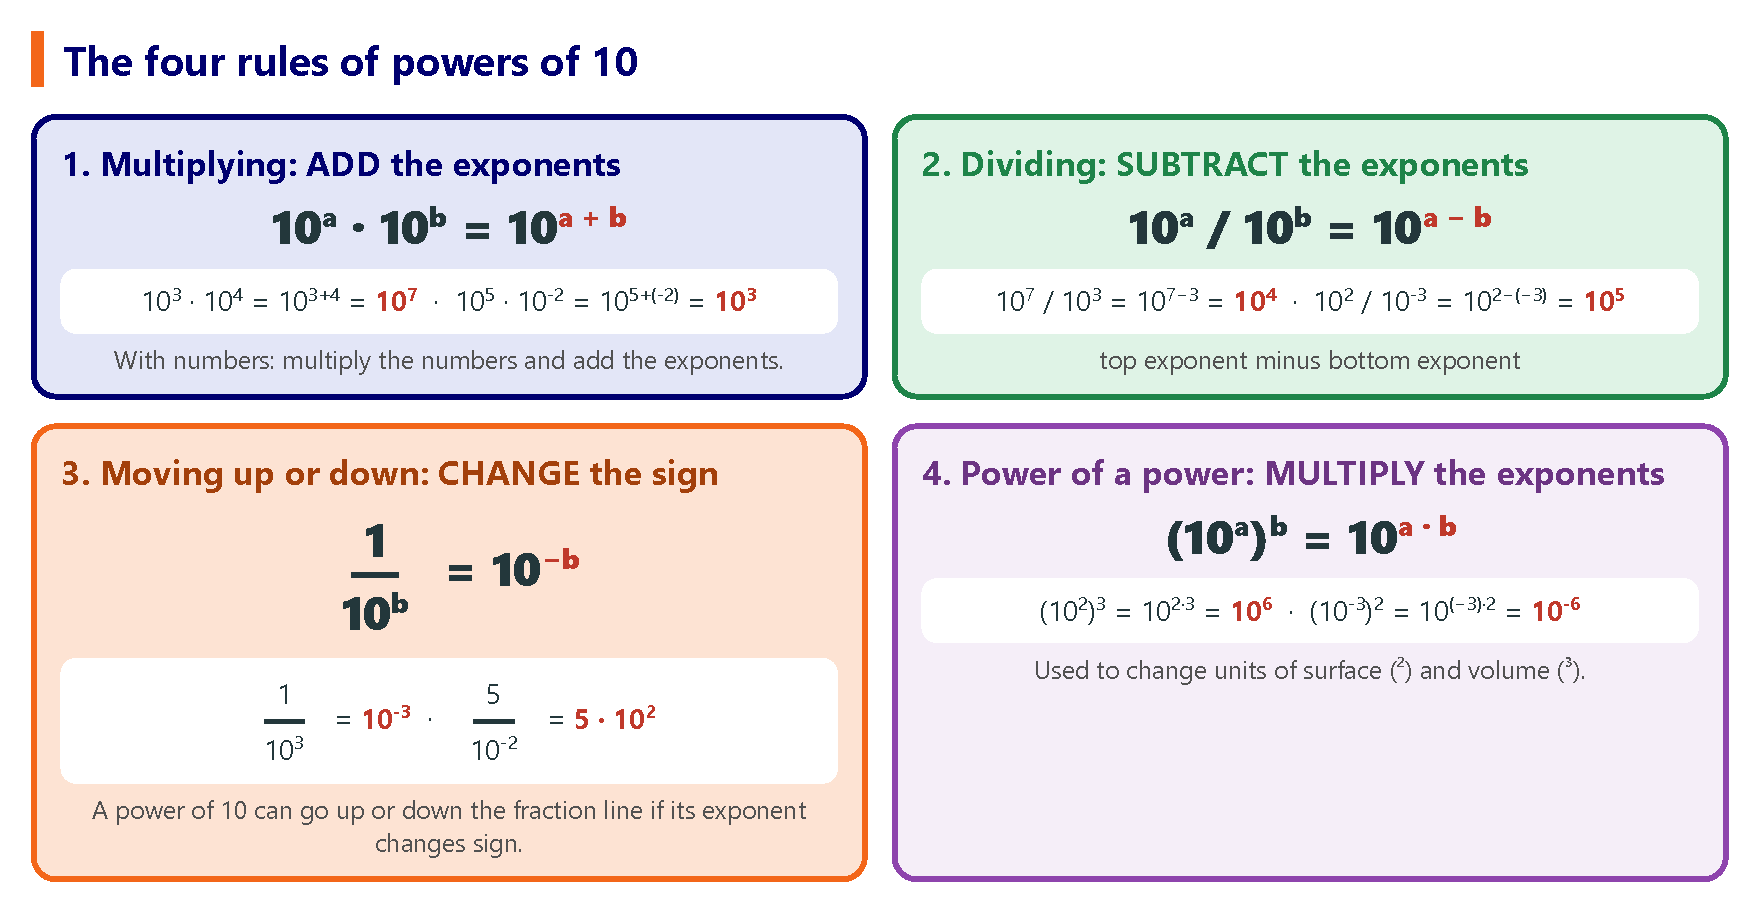
\includegraphics[width=\textwidth]{FigurasSVG/Unit_0_Math_Tools/pdf/power10_rules.pdf}
    \caption{The four rules for operating with powers of 10.}
    \label{fig:u0_power10_rules}
\end{figure}

\subsubsection{Multiplying: we add the exponents}

\begin{equation*}
    10^{a} \cdot 10^{b} = 10^{a+b}
\end{equation*}

If the powers of 10 have a number in front, we multiply the numbers on one side and the powers of 10 on the other:

\begin{example}
    \begin{itemize}
        \item \(10^{3} \cdot 10^{5} = 10^{3+5} = \textcolor{red}{10^{8}}\)
        \item \(10^{6} \cdot 10^{-2} = 10^{6+(-2)} = \textcolor{red}{10^{4}}\)
        \item \((3 \cdot 10^{4}) \cdot (2 \cdot 10^{3}) = (3 \cdot 2) \cdot 10^{4+3} = \textcolor{red}{6 \cdot 10^{7}}\)
        \item \((5 \cdot 10^{-3}) \cdot (4 \cdot 10^{6}) = 20 \cdot 10^{3} = \textcolor{red}{2 \cdot 10^{4}}\)
    \end{itemize}
\end{example}

\subsubsection{Dividing: we subtract the exponents}

\begin{equation*}
    \dfrac{10^{a}}{10^{b}} = 10^{a-b}
\end{equation*}

We subtract: exponent of the top \textbf{minus} exponent of the bottom. Be careful with the signs!

\begin{example}
    \begin{itemize}
        \item \(\dfrac{10^{8}}{10^{3}} = 10^{8-3} = \textcolor{red}{10^{5}}\)
        \item \(\dfrac{10^{2}}{10^{-4}} = 10^{2-(-4)} = 10^{2+4} = \textcolor{red}{10^{6}}\)
        \item \(\dfrac{8 \cdot 10^{6}}{2 \cdot 10^{2}} = \dfrac{8}{2} \cdot 10^{6-2} = \textcolor{red}{4 \cdot 10^{4}}\)
        \item \(\dfrac{9 \cdot 10^{-3}}{3 \cdot 10^{2}} = 3 \cdot 10^{-3-2} = \textcolor{red}{3 \cdot 10^{-5}}\)
    \end{itemize}
\end{example}

\subsubsection{Moving a power of 10 up or down: we change the sign of the exponent}

A power of 10 that is \textbf{below} the fraction line can be moved \textbf{above} it (and the other way round) if we \textbf{change the sign} of its exponent:
\begin{equation*}
    \dfrac{1}{10^{b}} = 10^{-b}
    \qquad\qquad
    10^{-b} = \dfrac{1}{10^{b}}
\end{equation*}

\begin{figure}[H]
    \centering
    % [FIGURA ORIGINAL] \includegraphics[width=\textwidth]{Unit_0/power10_flip}
    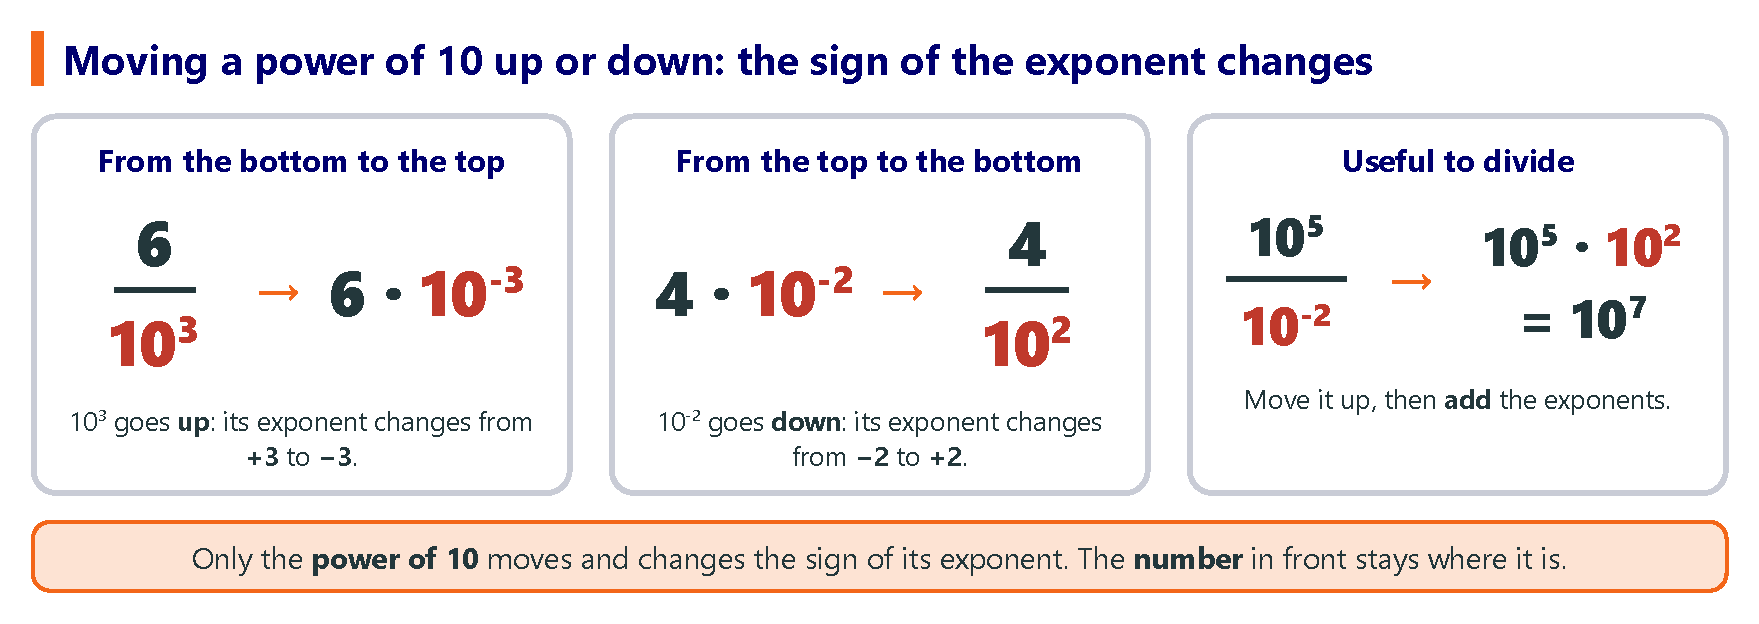
\includegraphics[width=\textwidth]{FigurasSVG/Unit_0_Math_Tools/pdf/power10_flip.pdf}
    \caption{When a power of 10 crosses the fraction line, its exponent changes sign.}
    \label{fig:u0_power10_flip}
\end{figure}

\begin{example}
    \begin{itemize}
        \item \(\dfrac{6}{10^{3}} = \textcolor{red}{6 \cdot 10^{-3}}\) \quad (\(10^{3}\) goes up as \(10^{-3}\))
        \item \(\dfrac{7}{10^{-2}} = \textcolor{red}{7 \cdot 10^{2}}\) \quad (\(10^{-2}\) goes up as \(10^{2}\))
        \item \(\dfrac{10^{5}}{10^{-2}} = 10^{5} \cdot 10^{2} = \textcolor{red}{10^{7}}\) \quad (we move it up and then add the exponents; it is the same result as subtracting \(5 - (-2) = 7\))
        \item This is very useful with conversion factors: \(\num{450}\,\unit{\mg} \cdot \dfrac{\qty{1}{\g}}{\qty{e3}{\mg}} = 450 \cdot 10^{-3}\,\unit{\g} = \qty{0.45}{\g}\).
    \end{itemize}
\end{example}

\subsubsection{Power of a power: we multiply the exponents}

\begin{equation*}
    \left(10^{a}\right)^{b} = 10^{a \cdot b}
\end{equation*}

If there is a number in front, it is also raised to the power: \(\left(3 \cdot 10^{2}\right)^{2} = 3^{2} \cdot 10^{2 \cdot 2} = 9 \cdot 10^{4}\).

\begin{example}
    \begin{itemize}
        \item \(\left(10^{3}\right)^{2} = 10^{3 \cdot 2} = \textcolor{red}{10^{6}}\)
        \item \(\left(10^{-2}\right)^{3} = 10^{(-2) \cdot 3} = \textcolor{red}{10^{-6}}\)
        \item \(\left(2 \cdot 10^{4}\right)^{3} = 2^{3} \cdot 10^{4 \cdot 3} = \textcolor{red}{8 \cdot 10^{12}}\)
        \item This is what we do when we change units of volume: \(\left(\dfrac{\qty{e2}{\cm}}{\qty{1}{\m}}\right)^{3} = \dfrac{10^{2 \cdot 3}\,\unit{\cubic\cm}}{\qty{1}{\cubic\m}} = \dfrac{\qty{e6}{\cubic\cm}}{\qty{1}{\cubic\m}}\).
    \end{itemize}
\end{example}

\begin{exercise}
    \textbf{Multiplying.} Calculate and leave the result as a power of 10:
    \begin{enumerate}[label=\letraminuscula]
        \item \(10^{4} \cdot 10^{2}\)
        \item \(10^{-3} \cdot 10^{-5}\)
        \item \(10^{7} \cdot 10^{-4}\)
        \item \((2 \cdot 10^{3}) \cdot (4 \cdot 10^{5})\)
        \item \((3 \cdot 10^{-2}) \cdot (3 \cdot 10^{6})\)
        \item \((5 \cdot 10^{4}) \cdot (6 \cdot 10^{-7})\)
    \end{enumerate}
    \begin{solu}
        a) \(10^{6}\); b) \(10^{-8}\); c) \(10^{3}\); d) \(8 \cdot 10^{8}\); e) \(9 \cdot 10^{4}\); f) \(30 \cdot 10^{-3} = 3 \cdot 10^{-2}\).
    \end{solu}
\end{exercise}

\begin{exercise}
    \textbf{Dividing.} Calculate and leave the result as a power of 10:
    \begin{enumerate}[label=\letraminuscula]
        \item \(\dfrac{10^{9}}{10^{4}}\)
        \item \(\dfrac{10^{3}}{10^{-2}}\)
        \item \(\dfrac{10^{-4}}{10^{2}}\)
        \item \(\dfrac{6 \cdot 10^{8}}{3 \cdot 10^{5}}\)
        \item \(\dfrac{8 \cdot 10^{-2}}{4 \cdot 10^{-6}}\)
        \item \(\dfrac{12 \cdot 10^{3}}{4 \cdot 10^{7}}\)
    \end{enumerate}
    \begin{solu}
        a) \(10^{5}\); b) \(10^{5}\); c) \(10^{-6}\); d) \(2 \cdot 10^{3}\); e) \(2 \cdot 10^{4}\); f) \(3 \cdot 10^{-4}\).
    \end{solu}
\end{exercise}

\begin{exercise}
    \textbf{Moving up.} Write without fractions, moving the power of 10 to the top:
    \begin{enumerate}[label=\letraminuscula]
        \item \(\dfrac{1}{10^{4}}\)
        \item \(\dfrac{3}{10^{2}}\)
        \item \(\dfrac{5}{10^{-3}}\)
        \item \(\dfrac{10^{2}}{10^{-5}}\)
    \end{enumerate}
    \begin{solu}
        a) \(10^{-4}\); b) \(3 \cdot 10^{-2}\); c) \(5 \cdot 10^{3}\); d) \(10^{2} \cdot 10^{5} = 10^{7}\).
    \end{solu}
\end{exercise}

\begin{exercise}
    \textbf{Power of a power.} Calculate:
    \begin{enumerate}[label=\letraminuscula]
        \item \(\left(10^{4}\right)^{2}\)
        \item \(\left(10^{-1}\right)^{3}\)
        \item \(\left(10^{-3}\right)^{-2}\)
        \item \(\left(3 \cdot 10^{2}\right)^{3}\)
        \item \(\left(\dfrac{\qty{e3}{\mm}}{\qty{1}{\m}}\right)^{2}\)
    \end{enumerate}
    \begin{solu}
        a) \(10^{8}\); b) \(10^{-3}\); c) \(10^{6}\); d) \(27 \cdot 10^{6} = 2{,}7 \cdot 10^{7}\); e) \(\dfrac{\qty{e6}{\square\mm}}{\qty{1}{\square\m}}\).
    \end{solu}
\end{exercise}

\begin{exercise}
    \textbf{Mixed.} Calculate, leaving the result as a power of 10, and then write it as a decimal number:
    \begin{enumerate}[label=\letraminuscula]
        \item \(\dfrac{10^{3} \cdot 10^{4}}{10^{5}}\)
        \item \(\dfrac{10^{-2} \cdot 10^{6}}{10^{-1}}\)
        \item \(\dfrac{(2 \cdot 10^{3})^{2}}{4 \cdot 10^{2}}\)
    \end{enumerate}
    \begin{solu}
        a) \(\dfrac{10^{7}}{10^{5}} = 10^{2} = 100\); \quad
        b) \(\dfrac{10^{4}}{10^{-1}} = 10^{5} = \num{100000}\); \quad
        c) \(\dfrac{4 \cdot 10^{6}}{4 \cdot 10^{2}} = 10^{4} = \num{10000}\).
    \end{solu}
\end{exercise}

%----------------------------------------------------------------------------------------

\section{Equations: how to isolate a quantity}

\subsection{What does isolating mean?}

In science, formulas link several quantities: \(d = \dfrac{m}{V}\), \(v = \dfrac{x}{t}\), \(F = m \cdot a\)\ldots{} Very often we know some of them and we want to calculate another one, which is not alone. Then we must \textbf{isolate} it.

\begin{definition}[Isolating a quantity]
    To \textbf{isolate} a quantity (\emph{despejar}) is to rearrange an equation so that this quantity is \textbf{completely alone} on one side of the equals sign, \textbf{in the numerator}, and everything else is on the other side.
\end{definition}

\begin{figure}[H]
    \centering
    % [FIGURA ORIGINAL] \includegraphics[width=\textwidth]{Unit_0/isolate_meaning}
    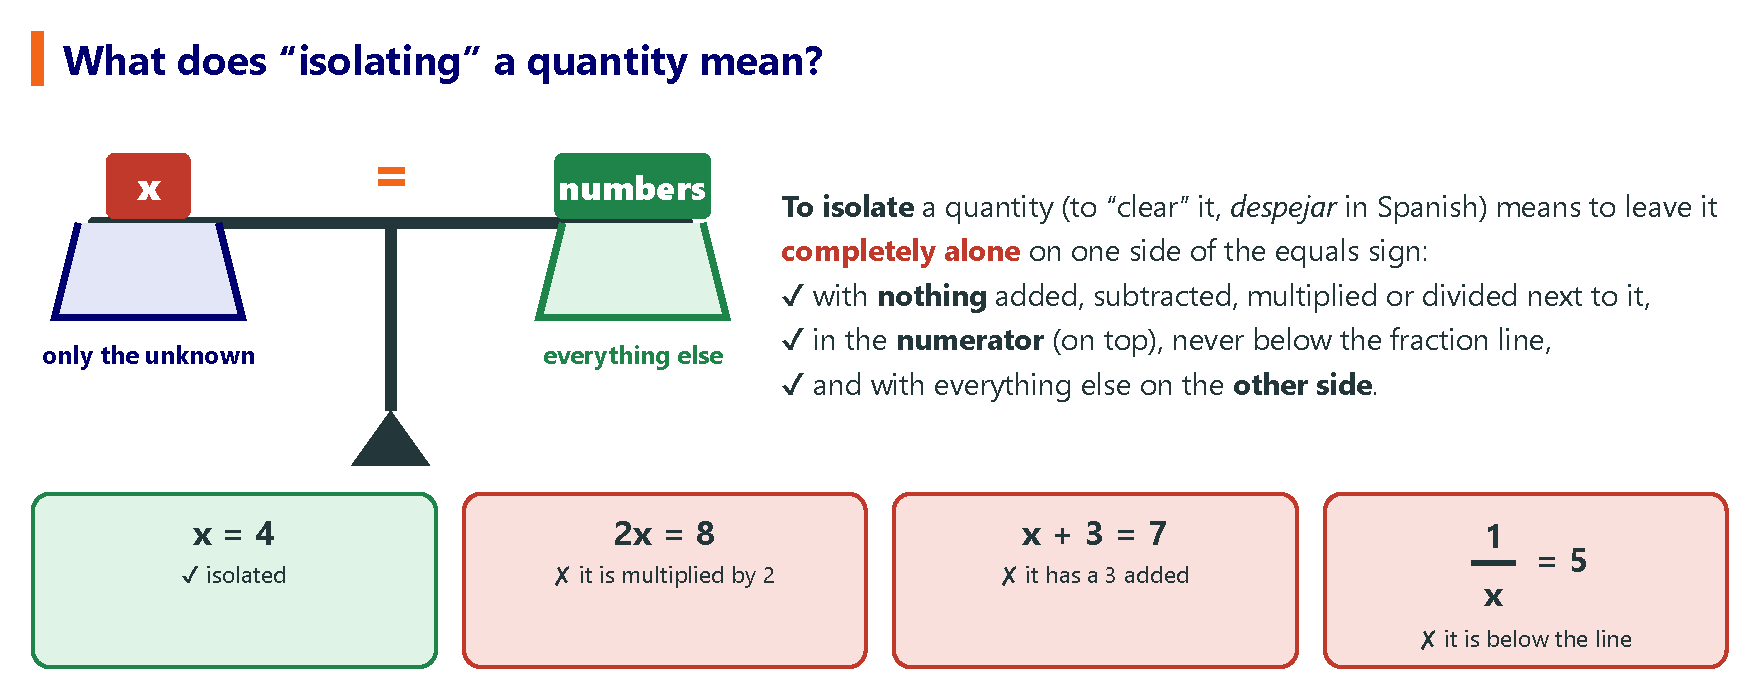
\includegraphics[width=\textwidth]{FigurasSVG/Unit_0_Math_Tools/pdf/isolate_meaning.pdf}
    \caption{An equation is like a balanced scale. Isolating means leaving the unknown alone on one side.}
    \label{fig:u0_isolate_meaning}
\end{figure}

An equation is like a \textbf{balanced scale}: the two sides are equal. If we do the \textbf{same operation on both sides}, the scale stays balanced and the equation is still true. We use this to remove, one by one, everything that is next to the unknown.

\subsection{Two methods to isolate}

\begin{figure}[H]
    \centering
    % [FIGURA ORIGINAL] \includegraphics[width=\textwidth]{Unit_0/isolate_shortcut}
    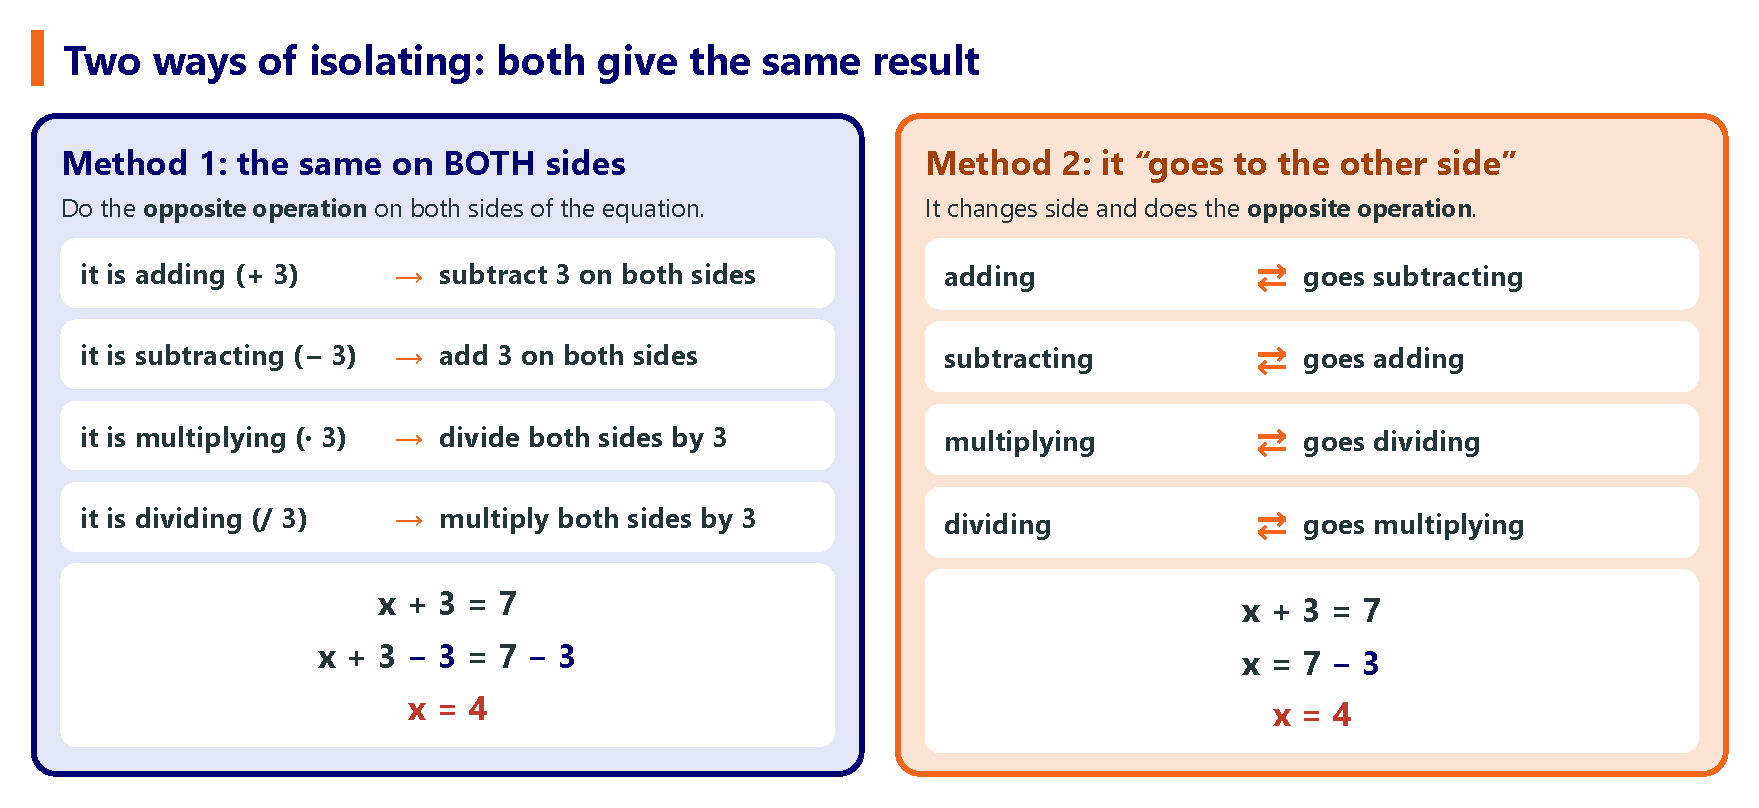
\includegraphics[width=\textwidth]{FigurasSVG/Unit_0_Math_Tools/pdf/isolate_shortcut.pdf}
    \caption{Method 1 (the same operation on both sides) and Method 2 (going to the other side) give the same result.}
    \label{fig:u0_isolate_shortcut}
\end{figure}

\negsubro{Method 1: the same operation on both sides} (the method of mathematics). We look at what is ``stuck'' to the unknown and we do the \textbf{opposite operation on both sides}:
\begin{itemize}
    \item If it is \textbf{adding}, we \textbf{subtract} it on both sides.
    \item If it is \textbf{subtracting}, we \textbf{add} it on both sides.
    \item If it is \textbf{multiplying}, we \textbf{divide} both sides by it.
    \item If it is \textbf{dividing}, we \textbf{multiply} both sides by it.
\end{itemize}

\negsubro{Method 2: going to the other side} (the shortcut). A quantity can \textbf{change side} if it also \textbf{changes its operation} to the opposite one:
\begin{center}
    \renewcommand{\arraystretch}{1.3}
    \begin{tabular}{ccc}
        \toprule
        \textbf{If it is\ldots} & & \textbf{it goes to the other side\ldots} \\
        \midrule
        adding \((+)\) & \(\longleftrightarrow\) & subtracting \((-)\) \\
        subtracting \((-)\) & \(\longleftrightarrow\) & adding \((+)\) \\
        multiplying \((\cdot)\) & \(\longleftrightarrow\) & dividing \((/)\) \\
        dividing \((/)\) & \(\longleftrightarrow\) & multiplying \((\cdot)\) \\
        \bottomrule
    \end{tabular}
\end{center}

\begin{impt}
    Method 2 is just a quick way of writing Method 1: when we ``pass'' the 3 subtracting, we are really subtracting 3 on both sides. Use the method you understand best, but \textbf{never} change the operation without changing the side!
\end{impt}

\subsection{Examples with both methods}

\begin{example}
    \textbf{Adding: \(x + 5 = 12\).}
    \begin{itemize}
        \item Method 1: we subtract 5 on both sides: \(x + 5 \textcolor{blue}{- 5} = 12 \textcolor{blue}{- 5}\) \(\Rightarrow\) \(\textcolor{red}{x = 7}\).
        \item Method 2: the 5 is adding, so it goes to the other side subtracting: \(x = 12 - 5\) \(\Rightarrow\) \(\textcolor{red}{x = 7}\).
    \end{itemize}
\end{example}

\begin{example}
    \textbf{Subtracting: \(x - 3 = 10\).}
    \begin{itemize}
        \item Method 1: we add 3 on both sides: \(x - 3 \textcolor{blue}{+ 3} = 10 \textcolor{blue}{+ 3}\) \(\Rightarrow\) \(\textcolor{red}{x = 13}\).
        \item Method 2: the 3 is subtracting, so it goes to the other side adding: \(x = 10 + 3\) \(\Rightarrow\) \(\textcolor{red}{x = 13}\).
    \end{itemize}
\end{example}

\begin{example}
    \textbf{Multiplying: \(4 \cdot x = 20\).}
    \begin{itemize}
        \item Method 1: we divide both sides by 4: \(\dfrac{\cancelred{4} \cdot x}{\cancelred{4}} = \dfrac{20}{4}\) \(\Rightarrow\) \(\textcolor{red}{x = 5}\).
        \item Method 2: the 4 is multiplying, so it goes to the other side dividing: \(x = \dfrac{20}{4}\) \(\Rightarrow\) \(\textcolor{red}{x = 5}\).
    \end{itemize}
\end{example}

\begin{example}
    \textbf{Dividing: \(\dfrac{x}{3} = 6\).}
    \begin{itemize}
        \item Method 1: we multiply both sides by 3: \(\dfrac{x \cdot \cancelred{3}}{\cancelred{3}} = 6 \cdot 3\) \(\Rightarrow\) \(\textcolor{red}{x = 18}\).
        \item Method 2: the 3 is dividing, so it goes to the other side multiplying: \(x = 6 \cdot 3\) \(\Rightarrow\) \(\textcolor{red}{x = 18}\).
    \end{itemize}
\end{example}

\begin{example}
    \textbf{Two steps: \(2 \cdot x + 3 = 11\).} First we remove what is \textbf{added or subtracted}, and then what is \textbf{multiplying or dividing}:
    \begin{enumerate}[label=\numberballmDarkTeal]
        \item The 3 is adding: it goes to the other side subtracting: \(2 \cdot x = 11 - 3 = 8\).
        \item The 2 is multiplying: it goes to the other side dividing: \(x = \dfrac{8}{2}\) \(\Rightarrow\) \(\textcolor{red}{x = 4}\).
        \item Check: \(2 \cdot 4 + 3 = 11\). \textcolor{green!50!black}{Correct!}
    \end{enumerate}
\end{example}

\begin{marker}
    \textbf{Always check your result}: put the value you have found back into the original equation. If both sides are equal, it is correct.
\end{marker}

\subsection{When the unknown is below the fraction line}

Sometimes the quantity we want to isolate is in the \textbf{denominator}, for example the time \(t\) in \(v = \dfrac{x}{t}\) or the volume \(V\) in \(d = \dfrac{m}{V}\). In this case, \textbf{the first step is always to bring it up}: we multiply both sides by it (it ``goes up multiplying'').

\begin{impt}
    If we do not bring the unknown up first, it stays in the denominator and what we get is \(\dfrac{1}{x}\), \textbf{not} \(x\). And \(\dfrac{1}{x}\) is \textbf{not} the same as \(x\): if \(\dfrac{1}{x} = 0{,}25\), then \(x = 4\), not \(0{,}25\)!
\end{impt}

\begin{figure}[H]
    \centering
    % [FIGURA ORIGINAL] \includegraphics[width=\textwidth]{Unit_0/denominator_up}
    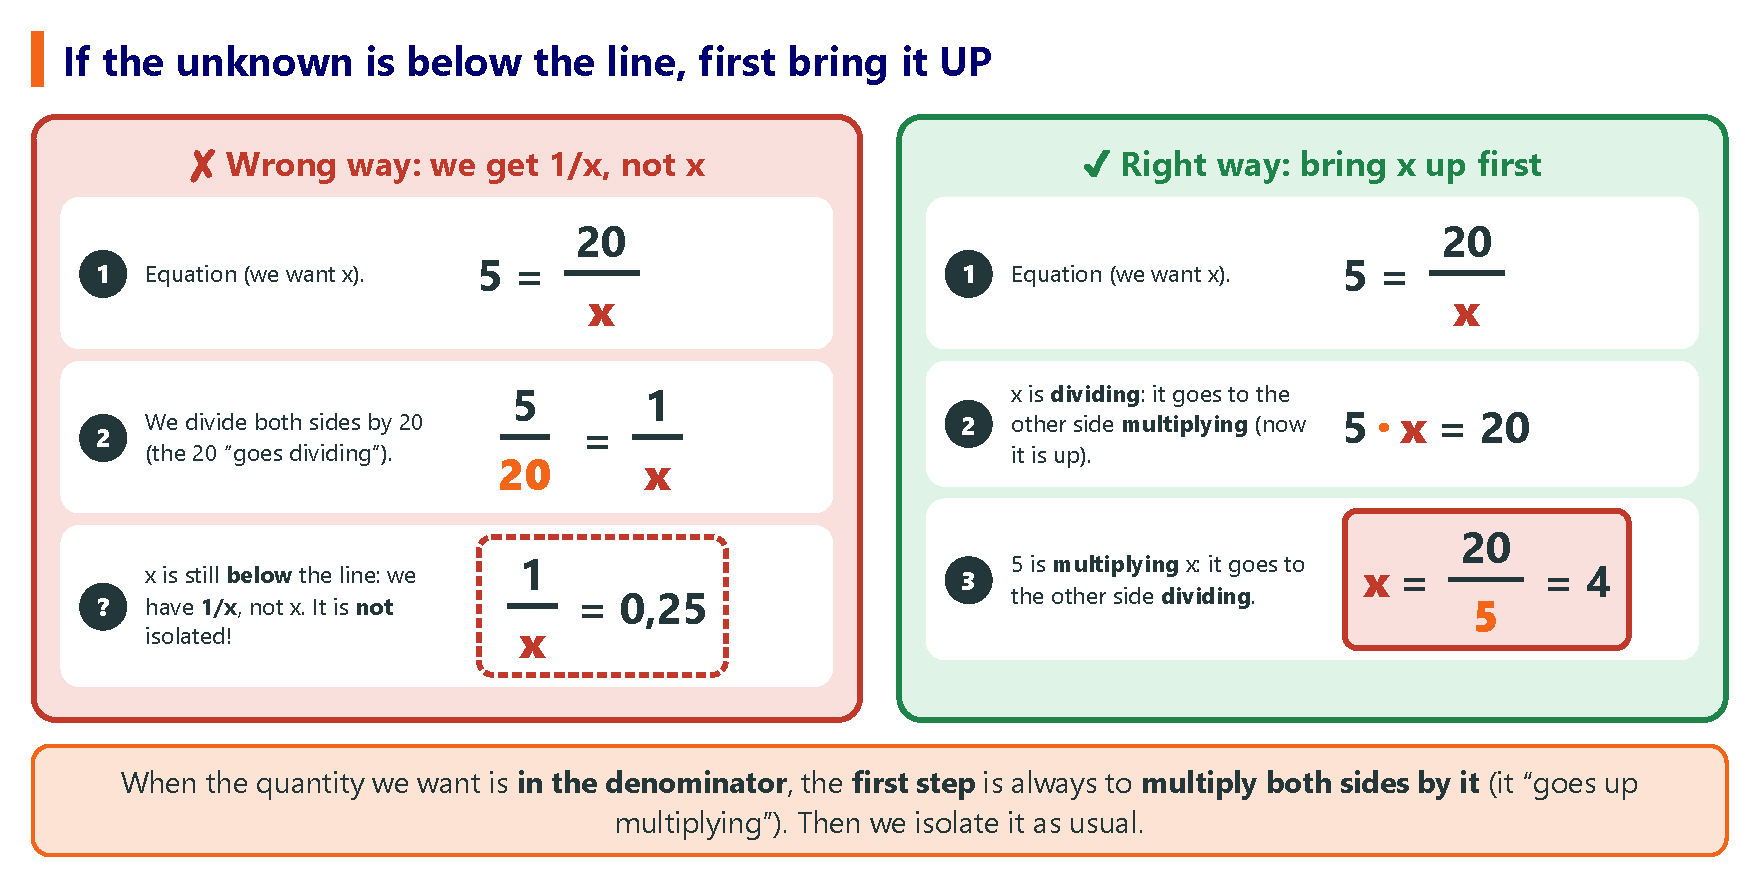
\includegraphics[width=\textwidth]{FigurasSVG/Unit_0_Math_Tools/pdf/denominator_up.pdf}
    \caption{If the unknown is in the denominator, we must first bring it up (multiplying); otherwise we get 1/x instead of x.}
    \label{fig:u0_denominator_up}
\end{figure}

\begin{example}
    \textbf{Isolate \(t\) in \(v = \dfrac{x}{t}\).}
    \begin{enumerate}[label=\numberballmDarkTeal]
        \item \(t\) is below the line, dividing: we bring it up multiplying (we multiply both sides by \(t\)): \(v \cdot t = x\).
        \item Now \(v\) is multiplying \(t\): it goes to the other side dividing: \(\textcolor{red}{t = \dfrac{x}{v}}\).
    \end{enumerate}
\end{example}

\begin{example}
    \textbf{Isolate \(V\) in \(d = \dfrac{m}{V}\), and calculate it for \(m = \qty{60}{\g}\) and \(d = \qty{3}{\g\per\cubic\cm}\).}
    \begin{enumerate}[label=\numberballmDarkTeal]
        \item \(V\) is below the line: it goes up multiplying: \(d \cdot V = m\).
        \item \(d\) is multiplying \(V\): it goes to the other side dividing: \(V = \dfrac{m}{d}\).
        \item \(V = \dfrac{\qty{60}{\g}}{\qty{3}{\g\per\cubic\cm}} = \textcolor{red}{\qty{20}{\cubic\cm}}\).
    \end{enumerate}
\end{example}

\subsection{Isolating in the formulas of physics and chemistry}

The method is exactly the same with letters as with numbers. Here are the formulas you will use most this year, with each quantity isolated:

\begin{table}[H]
    \centering
    \renewcommand{\arraystretch}{2.2}
    \begin{tabular}{llll}
        \toprule
        \textbf{Formula} & \multicolumn{3}{l}{\textbf{Isolated quantities}} \\
        \midrule
         \(d = \dfrac{m}{V}\) & \(m = d \cdot V\) & \(V = \dfrac{m}{d}\) & \\
        \(v = \dfrac{x}{t}\) & \(x = v \cdot t\) & \(t = \dfrac{x}{v}\) & \\
        \(F = m \cdot a\) & \(m = \dfrac{F}{a}\) & \(a = \dfrac{F}{m}\) & \\
        \(W = m \cdot g\) & \(m = \dfrac{W}{g}\) & \(g = \dfrac{W}{m}\) & \\
        \(T = t_{\text{C}} + 273\) & \(t_{\text{C}} = T - 273\) & & \\
        \(p_1 \cdot V_1 = p_2 \cdot V_2\) & \(V_2 = \dfrac{p_1 \cdot V_1}{p_2}\) & \(p_2 = \dfrac{p_1 \cdot V_1}{V_2}\) & \\
        \bottomrule
    \end{tabular}
    \caption{The most common formulas of the course, with each quantity isolated.}
    \label{tab:u0_formulas}
\end{table}

\begin{example}
    \textbf{Isolate \(v_f\) in \(a = \dfrac{v_f - v_i}{t}\).} Here the unknown is inside a subtraction that is divided by \(t\):
    \begin{enumerate}[label=\numberballmDarkTeal]
        \item \(t\) is dividing the whole subtraction: it goes to the other side multiplying: \(a \cdot t = v_f - v_i\).
        \item \(v_i\) is subtracting: it goes to the other side adding: \(\textcolor{red}{v_f = v_i + a \cdot t}\).
    \end{enumerate}
\end{example}

\begin{exercise}
    Isolate \(x\), using \textbf{both} methods, and check your result:
    \begin{enumerate}[label=\letraminuscula]
        \item \(x + 8 = 15\)
        \item \(x - 6 = 2\)
        \item \(5 \cdot x = 35\)
        \item \(\dfrac{x}{4} = 7\)
        \item \(3 \cdot x - 4 = 11\)
        \item \(\dfrac{x}{2} + 1 = 9\)
    \end{enumerate}
    \begin{solu}
        a) \(x = 15 - 8 = 7\); b) \(x = 2 + 6 = 8\); c) \(x = \dfrac{35}{5} = 7\); d) \(x = 7 \cdot 4 = 28\); e) \(3x = 11 + 4 = 15\), \(x = 5\); f) \(\dfrac{x}{2} = 9 - 1 = 8\), \(x = 16\).
    \end{solu}
\end{exercise}

\begin{exercise}
    The unknown is in the denominator. Bring it up first, and then isolate it:
    \begin{enumerate}[label=\letraminuscula]
        \item \(6 = \dfrac{30}{x}\)
        \item \(\dfrac{12}{x} = 4\)
        \item \(0{,}5 = \dfrac{2}{x}\)
        \item \(\dfrac{100}{x} = 25\)
    \end{enumerate}
    \begin{solu}
        a) \(6x = 30\), \(x = 5\); b) \(12 = 4x\), \(x = 3\); c) \(0{,}5x = 2\), \(x = 4\); d) \(100 = 25x\), \(x = 4\).
    \end{solu}
\end{exercise}

\begin{exercise}
    Isolate the quantity in brackets:
    \begin{enumerate}[label=\letraminuscula]
        \item \(d = \dfrac{m}{V}\) \quad (\(m\)) and (\(V\))
        \item \(v = \dfrac{x}{t}\) \quad (\(x\)) and (\(t\))
        \item \(F = m \cdot a\) \quad (\(a\))
        \item \(T = t_{\text{C}} + 273\) \quad (\(t_{\text{C}}\))
        \item \(\dfrac{V_1}{T_1} = \dfrac{V_2}{T_2}\) \quad (\(V_2\)) and (\(T_2\))
        \item \(a = \dfrac{v_f - v_i}{t}\) \quad (\(t\))
    \end{enumerate}
    \begin{solu}
        \begin{enumerate}[label=\alph*)]
            \item \(m = d \cdot V\); \(V = \dfrac{m}{d}\).
            \item \(x = v \cdot t\); \(t = \dfrac{x}{v}\).
            \item \(a = \dfrac{F}{m}\).
            \item \(t_{\text{C}} = T - 273\).
            \item \(V_2 = \dfrac{V_1 \cdot T_2}{T_1}\); \(T_2 = \dfrac{V_2 \cdot T_1}{V_1}\) (cross-multiply first: \(V_1 \cdot T_2 = V_2 \cdot T_1\)).
            \item \(t\) is in the denominator: \(a \cdot t = v_f - v_i\), so \(t = \dfrac{v_f - v_i}{a}\).
        \end{enumerate}
    \end{solu}
\end{exercise}

\begin{exercise}
    Isolate the unknown and calculate:
    \begin{enumerate}[label=\letraminuscula]
        \item The mass of a stone with \(V = \qty{50}{\cubic\cm}\) and \(d = \qty{2.6}{\g\per\cubic\cm}\).
        \item The time a car moving at \(v = \qty{20}{\mps}\) takes to travel \(x = \qty{900}{\m}\).
        \item The acceleration of a \(\qty{40}{\kg}\) trolley pushed with \(F = \qty{100}{\newton}\).
    \end{enumerate}
    \begin{solu}
        a) \(m = d \cdot V = \qty{2.6}{\g\per\cubic\cm} \cdot \qty{50}{\cubic\cm} = \qty{130}{\g}\); \quad
        b) \(t = \dfrac{x}{v} = \dfrac{\qty{900}{\m}}{\qty{20}{\mps}} = \qty{45}{\s}\); \quad
        c) \(a = \dfrac{F}{m} = \dfrac{\qty{100}{\newton}}{\qty{40}{\kg}} = \qty{2.5}{\mpss}\).
    \end{solu}
\end{exercise}

%----------------------------------------------------------------------------------------

\section{Graphs}

\subsection{The axes of a graph}

A graph has two perpendicular lines, called \textbf{axes}, that cross at the \textbf{origin} (0, 0):
\begin{itemize}
    \item The \textbf{horizontal axis} (in mathematics, the \(x\)-axis or \textbf{abscissa}).
    \item The \textbf{vertical axis} (in mathematics, the \(y\)-axis or \textbf{ordinate}).
\end{itemize}
Each point of the graph is written as \((\text{horizontal value}, \text{vertical value})\): the point \((3, 5)\) is 3 units to the right and 5 units up.

\begin{impt}
    \negsubro{In science, the axes do not have to be called \(x\) and \(y\)}. Each axis takes the name (and the unit) of the \textbf{quantity} we represent on it: \(t\) (s), \(v\) (m/s), \(m\) (g), \(T\) (\unit{\celsius})\ldots{} When we say ``\textbf{A vs B}'' (A \emph{versus} B), \textbf{A goes on the vertical axis} and \textbf{B goes on the horizontal axis}:
    \begin{itemize}
        \item ``\(v\) vs \(t\)'': \(v\) on the vertical axis and \(t\) on the horizontal axis.
        \item ``\(x\) vs \(t\)'': \(x\) on the vertical axis and \(t\) on the horizontal axis. Be careful: here \(x\) goes on the \textbf{vertical} axis!
        \item ``\(m\) vs \(V\)'': \(m\) on the vertical axis and \(V\) on the horizontal axis.
    \end{itemize}
    The time is almost always on the \textbf{horizontal} axis.
\end{impt}

\begin{figure}[H]
    \centering
    % [FIGURA ORIGINAL] \includegraphics[width=\textwidth]{Unit_0/axes_names}
    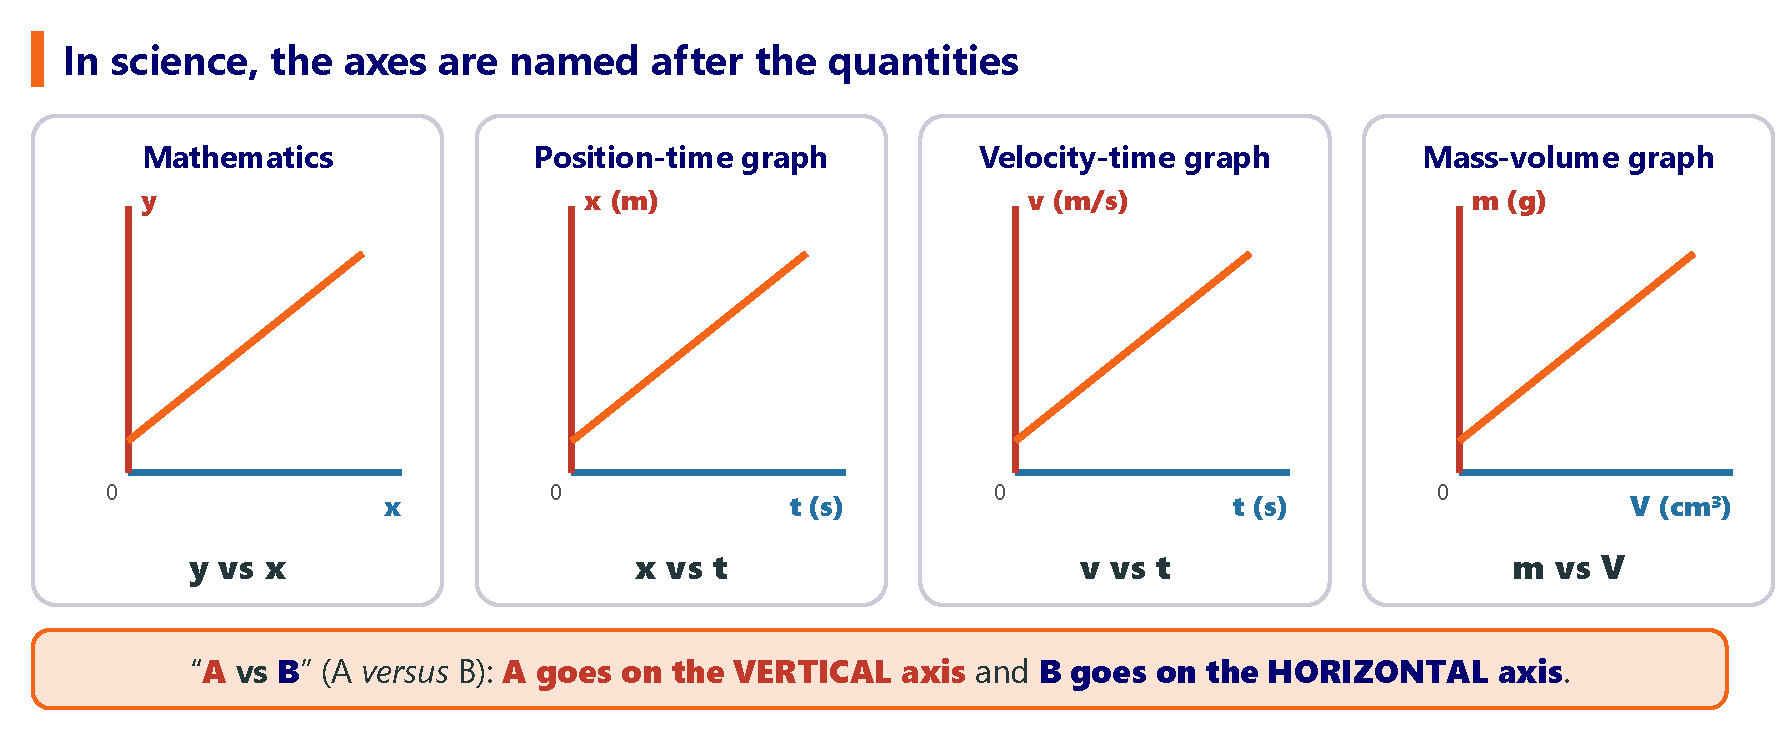
\includegraphics[width=\textwidth]{FigurasSVG/Unit_0_Math_Tools/pdf/axes_names.pdf}
    \caption{The same kind of graph with the axes named after different quantities.}
    \label{fig:u0_axes_names}
\end{figure}

\subsection{How to draw a graph from a table}

\negsubro{Method, step by step}:
\begin{enumerate}[label=\numberballmDarkTeal]
    \item Decide which quantity goes on each axis (``A vs B'': A vertical, B horizontal).
    \item Draw the axes and \textbf{label} them with the name of the quantity and its \textbf{unit}.
    \item Choose a \textbf{scale} for each axis, with equal steps (for example, every square is 2 s), so that all the values of the table fit.
    \item Plot each pair of values of the table as a \textbf{point}.
    \item If the points are in a straight line, join them with a \textbf{ruler}.
\end{enumerate}

\begin{example}
    \textbf{Mathematics: draw the graph of \(y = 2x + 1\).} First we make a table, giving values to \(x\):
    \begin{center}
        \begin{tabular}{lccccc}
            \toprule
            \(x\) & 0 & 1 & 2 & 3 & 4 \\
            \midrule
            \(y = 2x + 1\) & 1 & 3 & 5 & 7 & 9 \\
            \bottomrule
        \end{tabular}
    \end{center}
    \begin{center}
        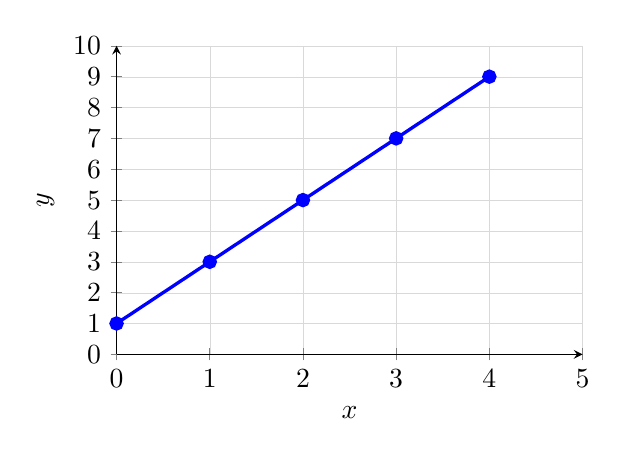
\begin{tikzpicture}
            \begin{axis}[width=7.5cm, height=5.5cm, grid=both, grid style={line width=.1pt, draw=gray!30},
                axis lines=left, xlabel={\(x\)}, ylabel={\(y\)}, xmin=0, xmax=5, ymin=0, ymax=10, xtick={0,1,...,5}, ytick={0,1,...,10}]
                \addplot[very thick, blue, mark=*] coordinates {(0,1) (1,3) (2,5) (3,7) (4,9)};
            \end{axis}
        \end{tikzpicture}
    \end{center}
\end{example}

\begin{example}
    \textbf{Science: draw the graph \(m\) vs \(V\) for pieces of aluminium.} Now the axes are called \(m\) (vertical) and \(V\) (horizontal), and each one has its unit:
    \begin{center}
        \begin{tabular}{lccccc}
            \toprule
            \(V\) (\unit{\cubic\cm}) & 0 & 10 & 20 & 30 & 40 \\
            \midrule
            \(m\) (\unit{\g}) & 0 & 27 & 54 & 81 & 108 \\
            \bottomrule
        \end{tabular}
    \end{center}
    \begin{center}
        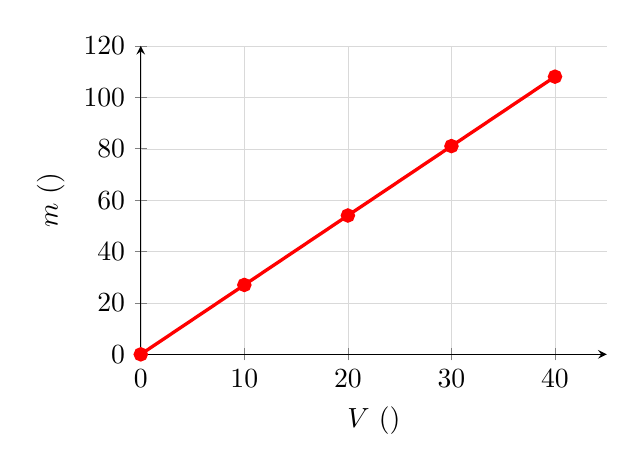
\begin{tikzpicture}
            \begin{axis}[width=7.5cm, height=5.5cm, grid=both, grid style={line width=.1pt, draw=gray!30},
                axis lines=left, xlabel={\(V\) (\unit{\cubic\cm})}, ylabel={\(m\) (\unit{\g})}, xmin=0, xmax=45, ymin=0, ymax=120, xtick={0,10,...,40}, ytick={0,20,...,120}]
                \addplot[very thick, red, mark=*] coordinates {(0,0) (10,27) (20,54) (30,81) (40,108)};
            \end{axis}
        \end{tikzpicture}
    \end{center}
    It is a straight line through the origin: the mass and the volume are \textbf{directly proportional}.
\end{example}

\subsection{Analysing straight-line graphs}

To read a straight-line graph we ask three questions:

\begin{figure}[H]
    \centering
    % [FIGURA ORIGINAL] \includegraphics[width=\textwidth]{Unit_0/slope}
    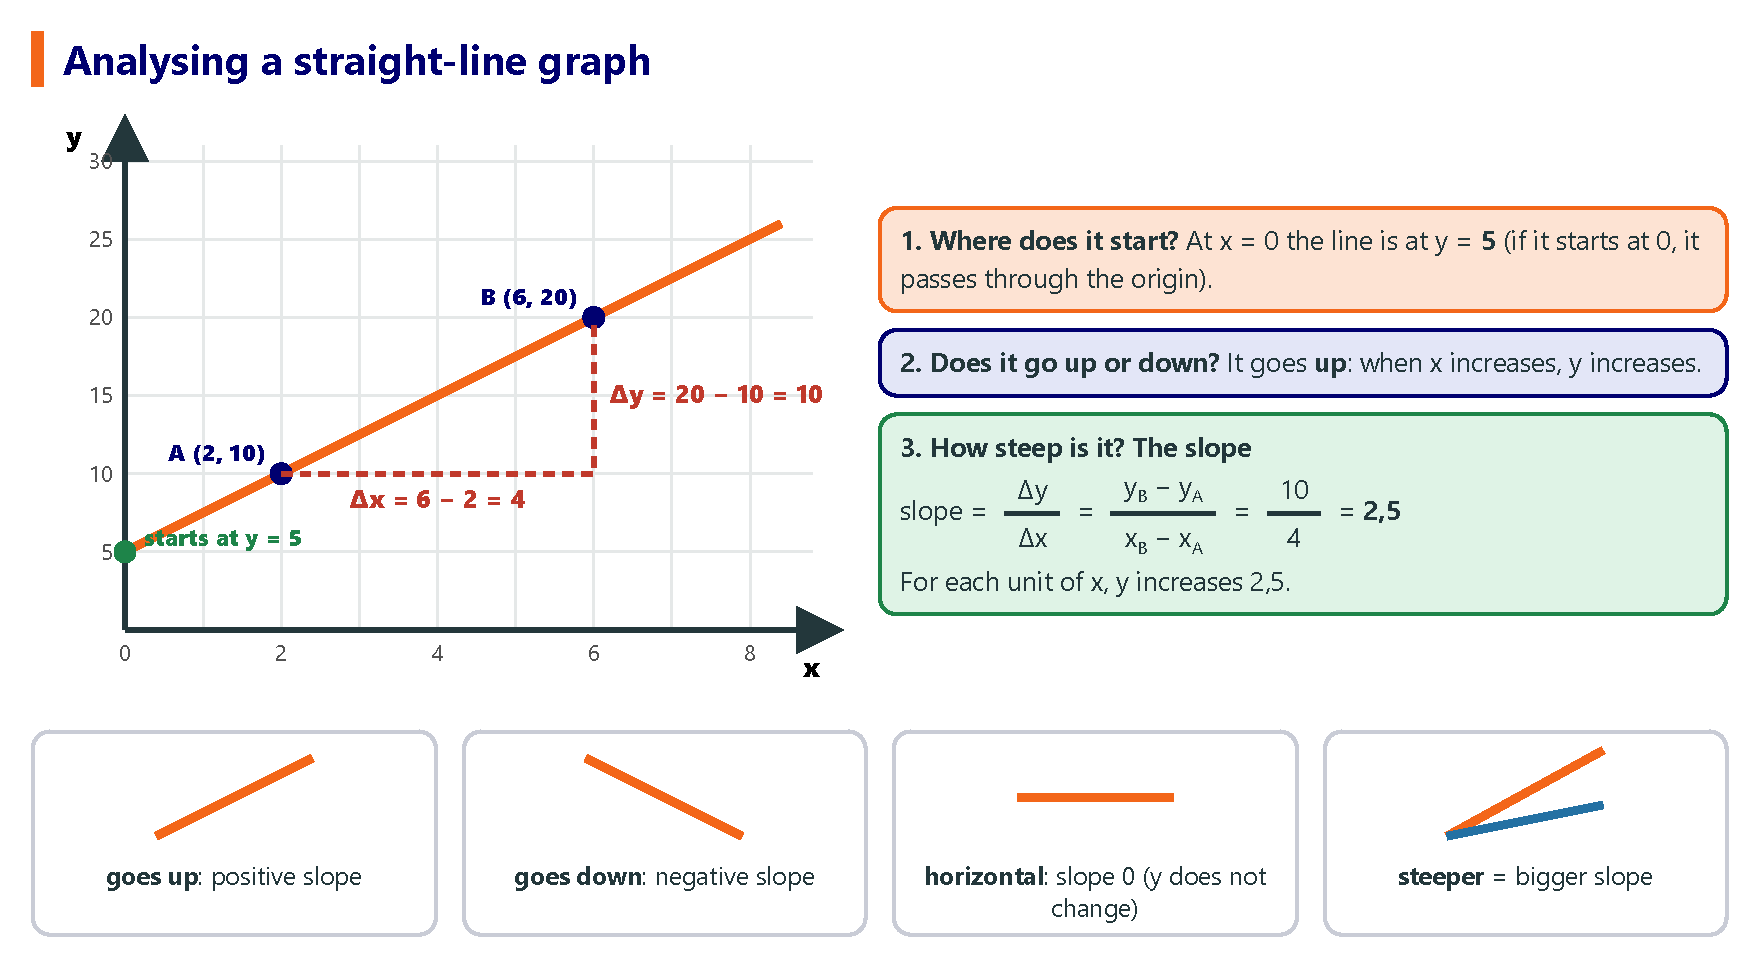
\includegraphics[width=\textwidth]{FigurasSVG/Unit_0_Math_Tools/pdf/slope.pdf}
    \caption{Where it starts, whether it goes up or down, and its slope.}
    \label{fig:u0_slope}
\end{figure}

\begin{enumerate}[label=\numberballmDarkTeal]
    \item \textbf{Where does it start?} The value on the vertical axis when the horizontal one is 0. If the line passes through \((0, 0)\), it starts at the \textbf{origin}.
    \item \textbf{Does it go up, go down or stay horizontal?} Going up means that the vertical quantity \textbf{increases}; going down, that it \textbf{decreases}; horizontal, that it \textbf{does not change}.
    \item \textbf{How steep is it?} This is the \negsubro{slope}: how much the vertical quantity changes for each unit of the horizontal one. We take two points \(A\) and \(B\) of the line:
    \begin{equation*}
        \text{slope} = \dfrac{\Delta(\text{vertical})}{\Delta(\text{horizontal})} = \dfrac{y_B - y_A}{x_B - x_A}
    \end{equation*}
\end{enumerate}

\begin{impt}
    \negsubro{In science the slope has a meaning}, and a unit:
    \begin{itemize}
        \item Slope of an \(x\) vs \(t\) graph \(= \dfrac{\Delta x}{\Delta t}\) = \textbf{velocity} (\unit{\mps}).
        \item Slope of a \(v\) vs \(t\) graph \(= \dfrac{\Delta v}{\Delta t}\) = \textbf{acceleration} (\unit{\mpss}).
        \item Slope of an \(m\) vs \(V\) graph \(= \dfrac{\Delta m}{\Delta V}\) = \textbf{density} (\unit{\g\per\cubic\cm}).
    \end{itemize}
\end{impt}

\begin{example}
    \textbf{In the aluminium graph above, calculate the slope and say what it means.} We take \(A = (10, 27)\) and \(B = (30, 81)\):
    \begin{equation*}
        \text{slope} = \dfrac{\qty{81}{\g} - \qty{27}{\g}}{\qty{30}{\cubic\cm} - \qty{10}{\cubic\cm}} = \dfrac{\qty{54}{\g}}{\qty{20}{\cubic\cm}} = \textcolor{red}{\qty{2.7}{\g\per\cubic\cm}}
    \end{equation*}
    The slope of an \(m\) vs \(V\) graph is the \textbf{density}: aluminium has a density of \qty{2.7}{\g\per\cubic\cm}.
\end{example}

\begin{exercise}
    \textbf{Mathematics.} Make a table with \(x = 0, 1, 2, 3, 4\) and draw the graph of each line. Then say where it starts, whether it goes up or down, and calculate its slope:
    \begin{enumerate}[label=\letraminuscula]
        \item \(y = 3x\)
        \item \(y = x + 2\)
        \item \(y = 10 - 2x\)
    \end{enumerate}
    \begin{solu}
        \begin{enumerate}[label=\alph*)]
            \item Table: \(y = 0, 3, 6, 9, 12\). Starts at the origin, goes up, slope \(= \dfrac{12 - 0}{4 - 0} = 3\).
            \item Table: \(y = 2, 3, 4, 5, 6\). Starts at \(y = 2\), goes up, slope \(= \dfrac{6 - 2}{4 - 0} = 1\).
            \item Table: \(y = 10, 8, 6, 4, 2\). Starts at \(y = 10\), goes down, slope \(= \dfrac{2 - 10}{4 - 0} = -2\).
        \end{enumerate}
    \end{solu}
\end{exercise}

\begin{exercise}
    \textbf{Science.} A pot of water is heated and its temperature is measured every minute:
    \begin{center}
        \begin{tabular}{lcccccc}
            \toprule
            \(t\) (min) & 0 & 1 & 2 & 3 & 4 & 5 \\
            \midrule
            \(T\) (\unit{\celsius}) & 20 & 30 & 40 & 50 & 60 & 70 \\
            \bottomrule
        \end{tabular}
    \end{center}
    \begin{enumerate}[label=\letraminuscula]
        \item Draw the graph ``\(T\) vs \(t\)''. Which quantity goes on each axis?
        \item What is the initial temperature?
        \item Calculate the slope. What does it mean?
    \end{enumerate}
    \begin{solu}
        \begin{enumerate}[label=\alph*)]
            \item \(T\) on the vertical axis and \(t\) on the horizontal axis. The points form a straight line going up.
            \item \qty{20}{\celsius} (the value at \(t = 0\)).
            \item Slope \(= \dfrac{\qty{70}{\celsius} - \qty{20}{\celsius}}{\qty{5}{\minute} - \qty{0}{\minute}} = \qty{10}{\celsius}\) per minute: the temperature rises \qty{10}{\celsius} every minute.
        \end{enumerate}
    \end{solu}
\end{exercise}

\begin{exercise}
    Read the graph ``\(v\) vs \(t\)'' of a car and answer the questions.
    \begin{center}
        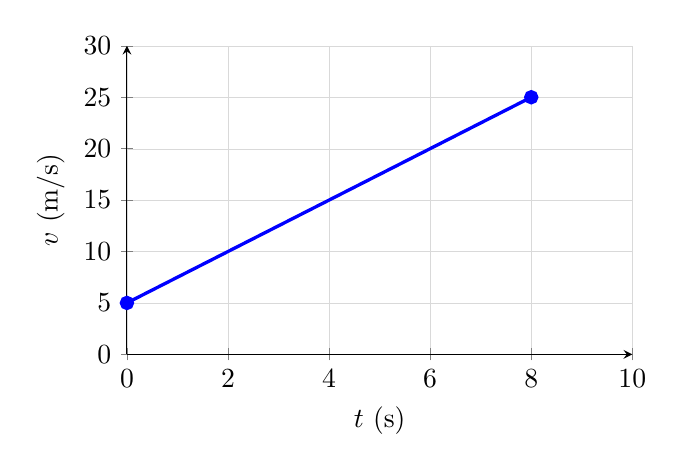
\begin{tikzpicture}
            \begin{axis}[width=8cm, height=5.5cm, grid=both, grid style={line width=.1pt, draw=gray!30},
                axis lines=left, xlabel={\(t\) (s)}, ylabel={\(v\) (m/s)}, xmin=0, xmax=10, ymin=0, ymax=30, xtick={0,2,...,10}, ytick={0,5,...,30}]
                \addplot[very thick, blue, mark=*] coordinates {(0,5) (8,25)};
            \end{axis}
        \end{tikzpicture}
    \end{center}
    \begin{enumerate}[label=\letraminuscula]
        \item Which quantity is on each axis?
        \item What is the velocity at \(t = 0\)? And at \(t = \qty{4}{\s}\)?
        \item Is the velocity increasing or decreasing?
        \item Calculate the slope. Which quantity is it?
    \end{enumerate}
    \begin{solu}
        \begin{enumerate}[label=\alph*)]
            \item \(v\) (m/s) on the vertical axis, \(t\) (s) on the horizontal axis.
            \item At \(t = 0\): \(v = \qty{5}{\mps}\). At \(t = \qty{4}{\s}\): \(v = \qty{15}{\mps}\).
            \item Increasing: the line goes up.
            \item Slope \(= \dfrac{\qty{25}{\mps} - \qty{5}{\mps}}{\qty{8}{\s} - \qty{0}{\s}} = \qty{2.5}{\mpss}\). It is the \textbf{acceleration}.
        \end{enumerate}
    \end{solu}
\end{exercise}

\begin{exercise}
    Draw, on the same axes, the graphs ``\(x\) vs \(t\)'' of two cyclists, using these tables. Who is faster? How do you see it on the graph?
    \begin{center}
        \begin{tabular}{lccccc}
            \toprule
            \(t\) (s) & 0 & 2 & 4 & 6 & 8 \\
            \midrule
            \(x_A\) (m) & 0 & 8 & 16 & 24 & 32 \\
            \(x_B\) (m) & 0 & 12 & 24 & 36 & 48 \\
            \bottomrule
        \end{tabular}
    \end{center}
    \begin{solu}
        Both are straight lines through the origin. Slope of \(A\): \(\dfrac{32}{8} = \qty{4}{\mps}\); slope of \(B\): \(\dfrac{48}{8} = \qty{6}{\mps}\). \(B\) is faster: its line is \textbf{steeper} (it has a bigger slope).
    \end{solu}
\end{exercise}

%----------------------------------------------------------------------------------------

\section*{Summary}

\begin{itemize}
    \item \textbf{Powers of 10}: \(10^{n}\) is a 1 followed by \(n\) zeros; \(10^{-n}\) has the 1 in the \(n\)-th decimal place; \(10^{0} = 1\).
    \item \textbf{Rules}: \(10^{a} \cdot 10^{b} = 10^{a+b}\); \(\dfrac{10^{a}}{10^{b}} = 10^{a-b}\); \(\dfrac{1}{10^{b}} = 10^{-b}\) (a power of 10 changes the sign of its exponent when it crosses the fraction line); \(\left(10^{a}\right)^{b} = 10^{a \cdot b}\).
    \item \textbf{Isolating} a quantity means leaving it alone, in the numerator, on one side of the equation. We do the opposite operation on both sides or, with the shortcut, it goes to the other side with the opposite operation.
    \item If the unknown is in the \textbf{denominator}, we first bring it up multiplying; otherwise we get \(1/x\), not \(x\).
    \item \textbf{Graphs}: ``A vs B'' means A on the vertical axis and B on the horizontal axis. A straight-line graph is described by where it starts, whether it goes up or down, and its \textbf{slope} \(= \Delta(\text{vertical}) / \Delta(\text{horizontal})\).
\end{itemize}
